%!TEX root = ../template.tex
%Developed using Sublime Text 3 with LaTexTools plugin
%SUPER+b for compiling latex to pdf
%Don't forget to use SUPER+R to jump between top level commands!
%F6 to spell check
%%%%%%%%%%%%%%%%%%%%%%%%%%%%%%%%%%%%%%%%%%%%%%%%%%%%%%%%%%%%%%%%%%%%
%% chapter2.tex
%% UNL thesis document file
%%
%% Chapter with the basics about three phase induction motors
%%%%%%%%%%%%%%%%%%%%%%%%%%%%%%%%%%%%%%%%%%%%%%%%%%%%%%%%%%%%%%%%%%%%
\chapter{Understanding Three Phase Induction Motors}
\label{cha:intro_electric_motors}

% ================
% = Introduction =
% ================


This chapter introduces the principal concepts that must be known when addressing \acrfull{tps}. Section \ref{sec:three_phase_systems} presents an overview of what is a \acrshort{tps} and its properties. Section \ref{sec:three_phase_induction_motors} explains the composition of a three phase \acrfull{em} - also known as \acrfull{tpim} - as well as its working principle and several properties and characteristics. In section \ref{sec:tpin_relevance} it is presented the reason why this kind of motor is so important and its landscape. Furthermore, section \ref{sec:Three_phase_induction_motors_maintenance_and_lyfe_cycle} will present the life cycle cost of these motors and approach the current maintenance strategies. The sources of the information presented in this chapter are mainly ~\cite{Helfenstein2000}, ~\cite{Alves2003}, ~\cite{Fitzgerald1985}, ~\cite{Guru2001}, ~\cite{Rashid2011} and ~\cite{Ferreira1}.

\section{Three phase Circuits} % (fold)
\label{sec:three_phase_systems}

A three-phase circuit is an \acrshort{ac}-circuit which contains three voltage power sources. These circuits have a power source with three phases and a three phase load that connects its phases to the power source phases. The generation of electric power in a three-phase system is accomplished with an electric generator, which converts mechanical energy to electric energy appropriated to this mode. Each phase has a sinusoidal voltage with a magnitude and frequency. An example of a three phase electric system schematic is represented in figure \ref{fig:balanced_tp_circuit}.

\begin{figure}[htbp]
	\centering
	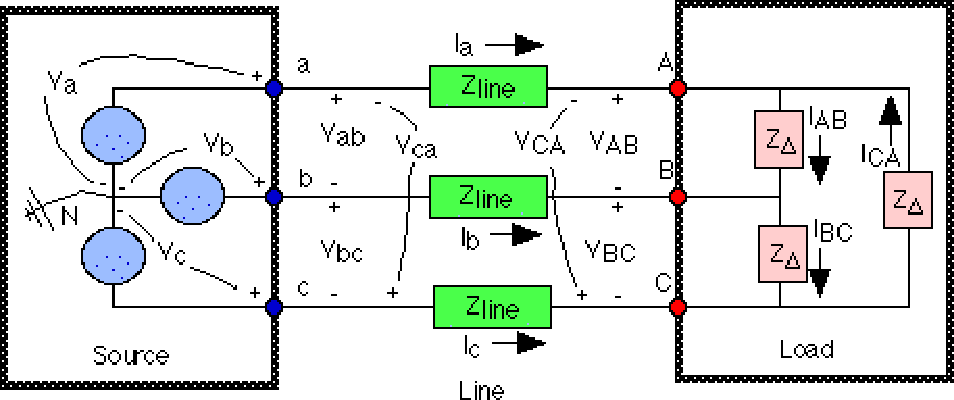
\includegraphics[height=2in]{3p3}
	\caption{A balanced three phase circuit with a load connected in $\Delta$}
	\label{fig:balanced_tp_circuit}
\end{figure}

\subsection{Motivation}

A three-phase circuit has several advantages over a single-phase circuit - and that's why the three-phase circuits have been adopted universally for transmission of AC power.

With a three-phase system we can get an higher power/weight ratio of alternators, since a three-phase alternator is smaller and lighter than a single phase alternator of the same power output. Also, the three-phase transmission system  requires less copper or aluminium to transmit the same quantity of power of a specific distance than a single phase system.

In single phase systems the instantaneous power is sinusoidal, therefore not constant, resulting in power vibrations. In a balanced three phase power system, though, the instantaneous power is always the same.

\subsection{Characteristics}

As the name implies, these circuits have a three-phase system voltage. If the sinusoidal voltages have the same magnitude and frequency and each voltage is 120º out of phase with the other two, the voltages are said to be balanced. If the loads are such that the currents produced by the voltages are also balanced, the entire circuit is referred to as a \emph{balanced three-phase circuit}.

\begin{figure}[htbp]
	\centering
	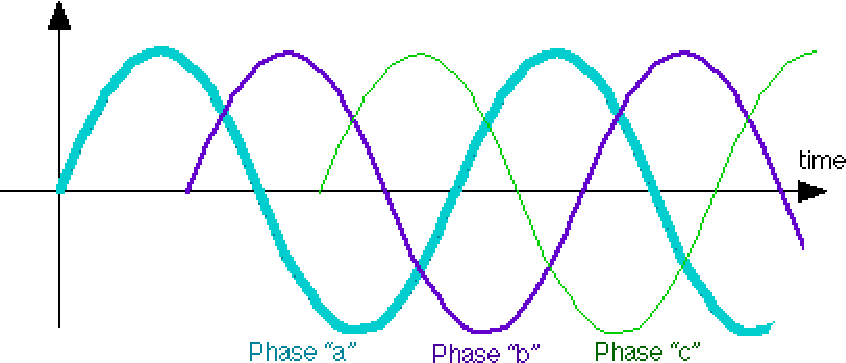
\includegraphics[height=2in]{threephase}
	\caption{Balanced 3-Phase Variables in Time Domain}
	\label{fig:balanced_tp_time_domain}
\end{figure}

Each phase is separated by 120º, which means that if phase \emph{a} has a value of 0 in 0º, then the phase \emph{b} will have a value of 0 in 0º + 120º and phase \emph{c} will have a value 0 in 0º + 120º + 120º, as in figure \ref{fig:balanced_tp_time_domain}. Given that the voltages represented in the figure are the difference between each phases' potential energy and neutral's potential energy, each phase can also be noted as phase \emph{an}, \emph{bn} and \emph{cn}.

\subsection{Line-to-neutral voltage phasors}

The voltage phases of figure \ref{fig:balanced_tp_time_domain} can be expressed in the time domain as:
\begin{equation} \label{eq:balanced_tpVan_timedomain}
	V_{an}(t) = V_{m}\sqrt{2}\cos{\omega t}
	\tagaddtext{V}
\end{equation}
\begin{equation} \label{eq:balanced_tpVbn_timedomain}
	V_{bn}(t) = V_{m}\sqrt{2}\cos{\left(\omega t - 120\degree\right)} 
	\tagaddtext{V}
\end{equation}
\begin{equation} \label{eq:balanced_tpVcn_timedomain}
	V_{cn}(t) = V_{m}\sqrt{2}\cos{\left(\omega t - 240\degree\right)} 
	\tagaddtext{V}
\end{equation}

where $V_{an}$ represents the voltage between phase \emph{a} and neutral, $V_{bn}$ represents the voltage between phase \emph{b} and neutral, $V_{cn}$ represents the voltage between phase \emph{c} and neutral, $V_{m}$ denotes the phasors' magnitude and $\omega$ represents the angular velocity - which is $2\pi f$, where $f$ is the frequency of the phase. 

These voltage phases can also be represented in phasors. A phasor is a complex number representing a sinusoidal function whose amplitude $(A)$ and initial phase $(\phi)$ are time-invariant - and can be noted as:

\begin{equation} \label{eq:balanced_tpVan}
	V_{an} = V_{m}\angle_{\phi}
\end{equation}
\begin{equation} \label{eq:balanced_tpVbn}
	V_{bn} = V_{m}\angle_{\omega - 120\degree} 
\end{equation}
\begin{equation} \label{eq:balanced_tpVcn}
	V_{cn} = V_{m}\angle_{\phi - 240\degree} = V_{m}\angle_{\phi + 120\degree} 
\end{equation}

\noindent where $\angle$ represents an angle, and $\phi$ represents the initial phase angle.

\begin{figure}[htbp]
	\centering
	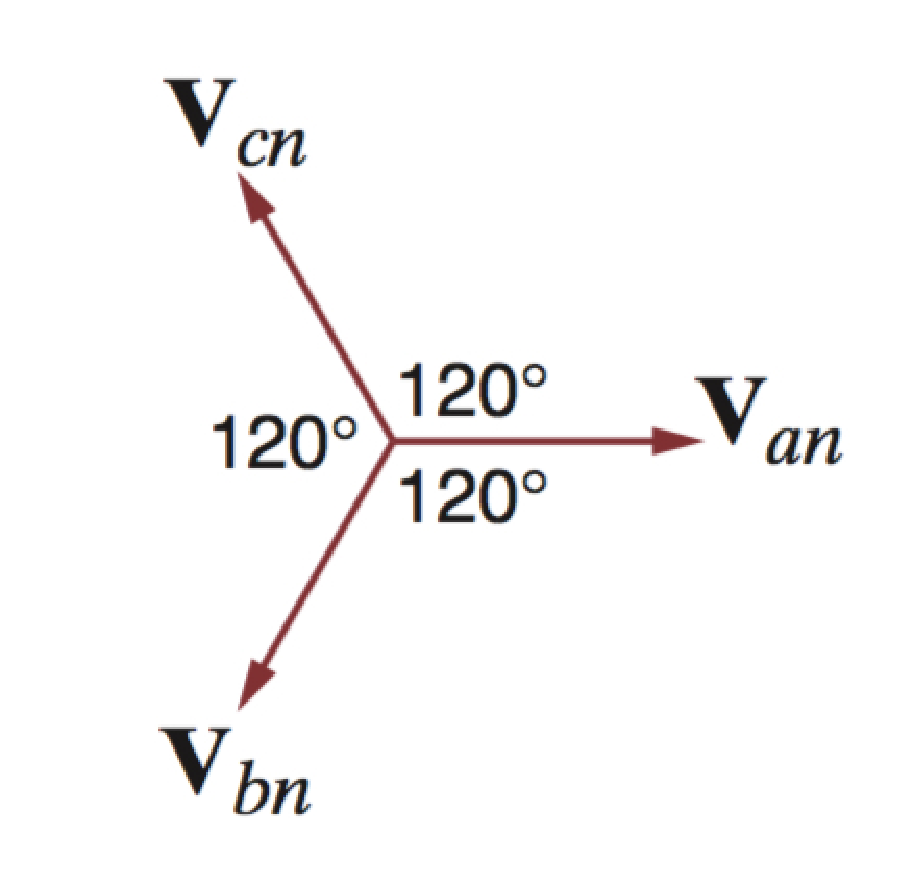
\includegraphics[height=2in]{phasorDiagramExample}
	\caption{Phasor diagram for a balanced three phase voltage source}
	\label{fig:balanced_tp_phasor_domain}
\end{figure}

Since the phasors have the same magnitude and are the same amount of degrees apart of each other, we can also represent them as follow:

\begin{equation} \label{eq:balanced_Vbn2}
	V_{bn} = V_{an}(1\angle_{-120\degree})
\end{equation}
\begin{equation} \label{eq:balanced_Vcn2}
	V_{cn} = V_{an}(1\angle_{+120\degree})
\end{equation}

These phasors can be represented on a phasor diagram, as shown in figure \ref{fig:balanced_tp_phasor_domain}. This potential difference between a given point (\emph{a},\emph{b} or \emph{c}) and the neutral is called the \emph{line-to-neutral voltage}. 
An important property of the balanced voltage phasors set is the following:
\begin{equation} \label{eq:balanced_prop1}
	V_{an} + V_{bn} + V_{cn} = 0
\end{equation}
as we can infer from figure \ref{fig:balanced_tp_phasor_domain}.

The magnitude of these phasors are typically measured in \acrfull{rms}, which is calculated by:
\begin{equation} \label{eq:rms}
	X_{rms} = \sqrt{\frac{1}{N}\sum\limits_{i=1}^{N}x_{i}^2}
\end{equation}

\subsection{Line-to-line voltage Phasors}

Besides the line-to-neutral voltage, there is also the line-to-line voltage - which is the potential difference between two phase lines.
In the phasor diagram, this can be seen as the sum of two phasors representing the phases, as shown in figure \ref{fig:line_to_line_phasors}.


\begin{figure}[htbp]
	\centering
	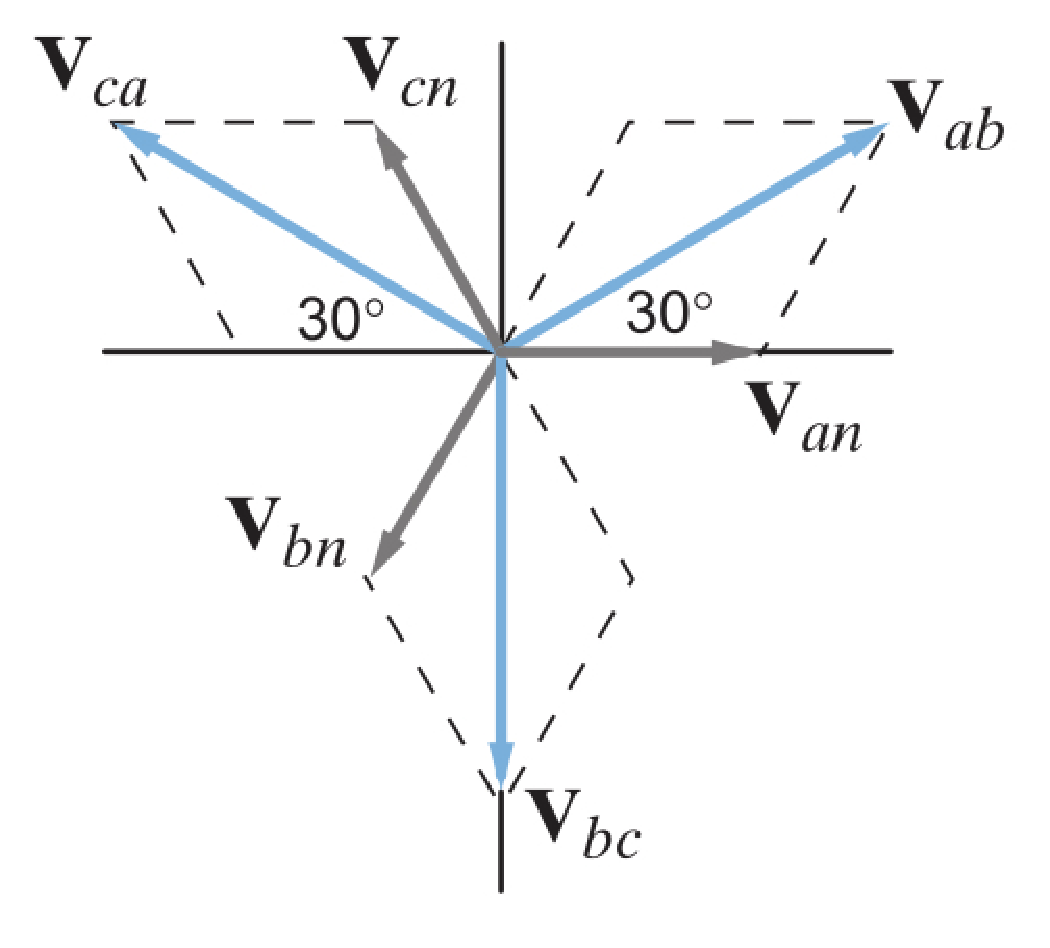
\includegraphics[height=2in]{linetolinephasor}
	\caption{Phasor representation of line-to-line voltages}
	\label{fig:line_to_line_phasors}
\end{figure}

We can obtain the set of line-to-line voltages as the following:

\begin{equation} \label{eq:balanced_tpVab}
	V_{ab} = \sqrt{3}V_{p}\angle_{\phi+30\degree}
\end{equation}
\begin{equation} \label{eq:balanced_tpVbc}
	V_{bc} = \sqrt{3}V_{p}\angle_{\phi - 120\degree + 30\degree} = \sqrt{3}V_{p}\angle_{\phi - 90\degree}
\end{equation}
\begin{equation} \label{eq:balanced_tpVca}
	V_{ca} = \sqrt{3}V_{p}\angle_{\phi - 240\degree + 30\degree} = \sqrt{3}V_{p}\angle_{\phi -210\degree} 
\end{equation}

where $V_{p}$ is the phase voltage magnitude (since the system is balanced, it can either be phase \emph{a}, \emph{b} or \emph{c}).

\subsection{Connection types}

From the standpoint of the user who connects a balanced load to the balanced three phase voltage source, there are two possible configurations for the load. The load can be connected in \emph{wye} (Y) - figure \ref{fig:wye_connected_load} -  or in \emph{delta} ($\Delta$) - figure \ref{fig:delta_connected_load}.

As you can notice from the figures \ref{fig:wye_connected_load} and \ref{fig:delta_connected_load}, these configurations differ in the way that Y connections are all connected to the line neutral, whereas the $\Delta$ connections are connected with each two other phase - being it phase \emph{a} connected to phase \emph{b}, phase \emph{b} connected to phase \emph{c} and phase \emph{c} connected to phase \emph{a}. Thus, connecting the load in Y configuration will create a line impedance of $Z_{Y}$, while connecting the load in $\Delta$ will create a line impedance of $Z_{\Delta}$.

\begin{figure}[htbp]
	\centering
	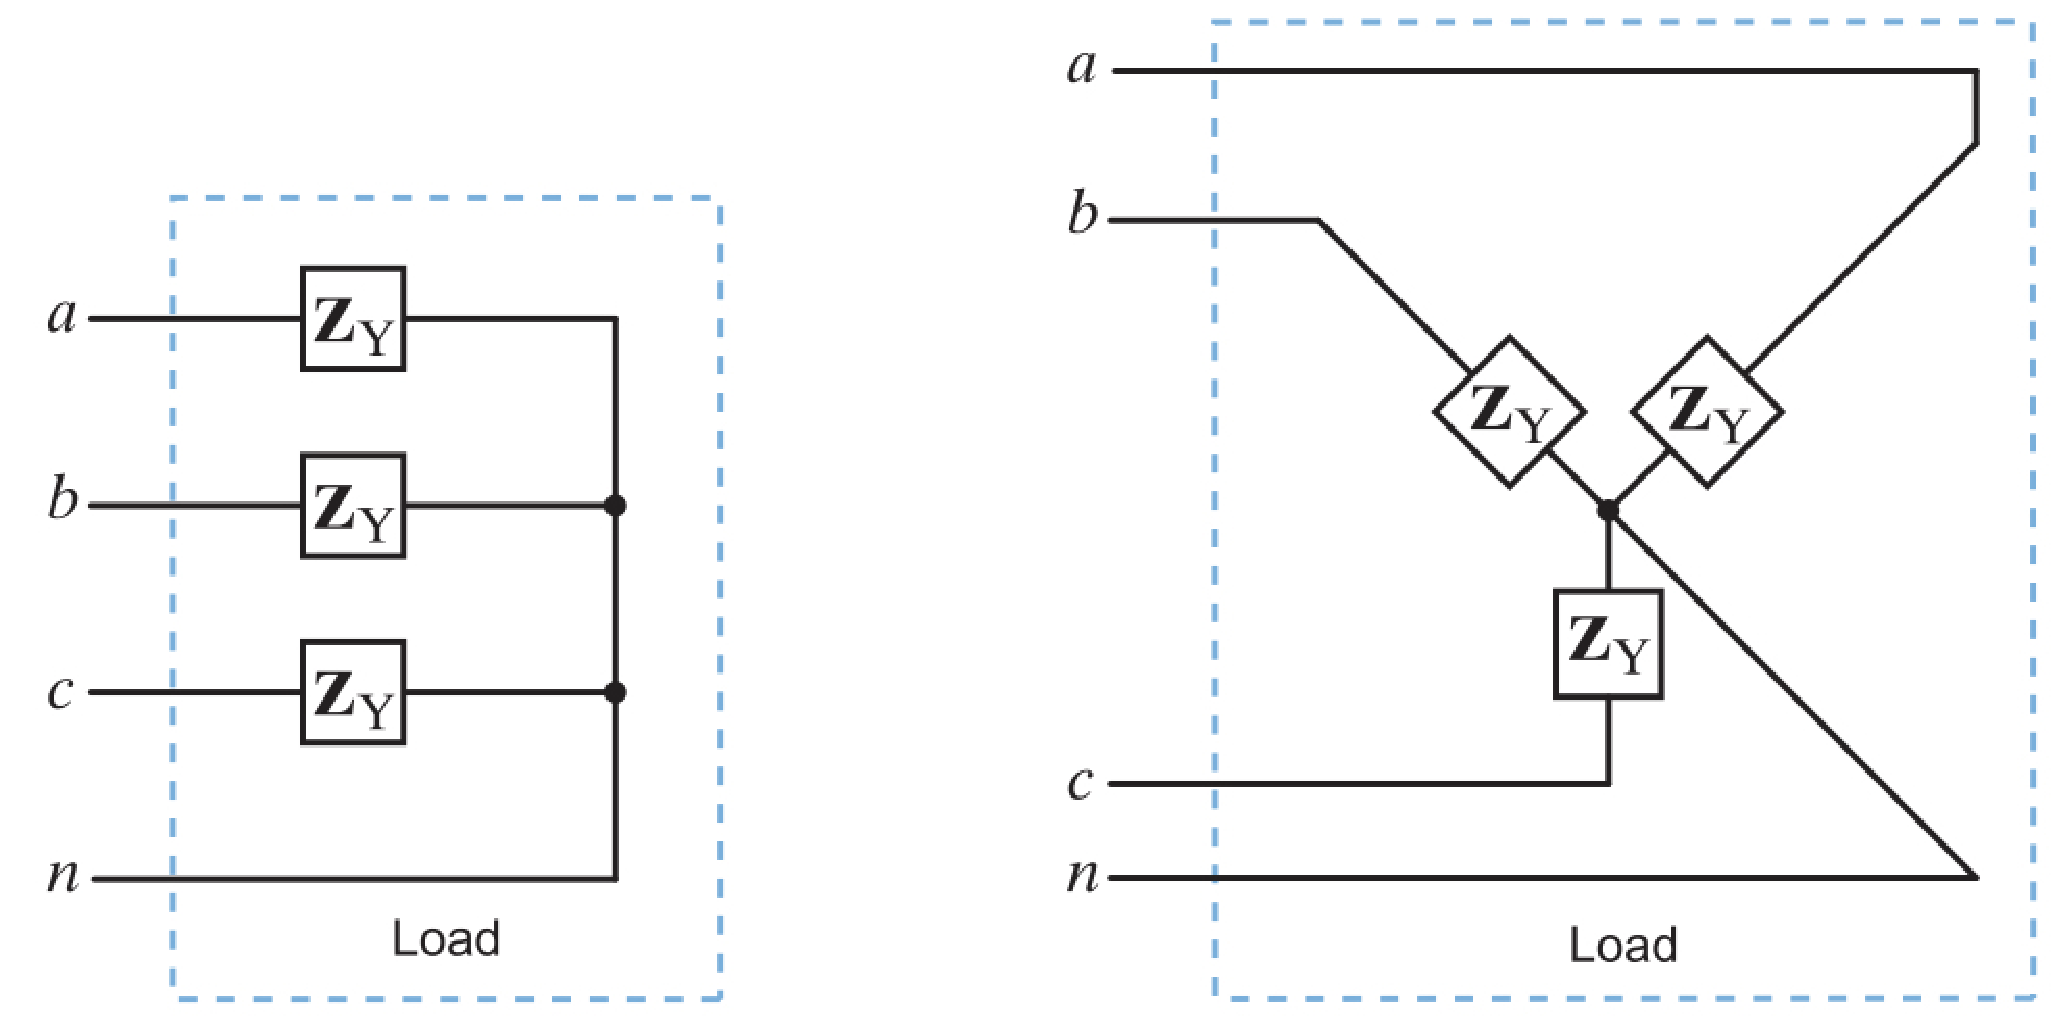
\includegraphics[height=2in]{wye_connection}
	\caption{Wye connected load}
	\label{fig:wye_connected_load}
\end{figure}

\begin{figure}[htbp]
	\centering
	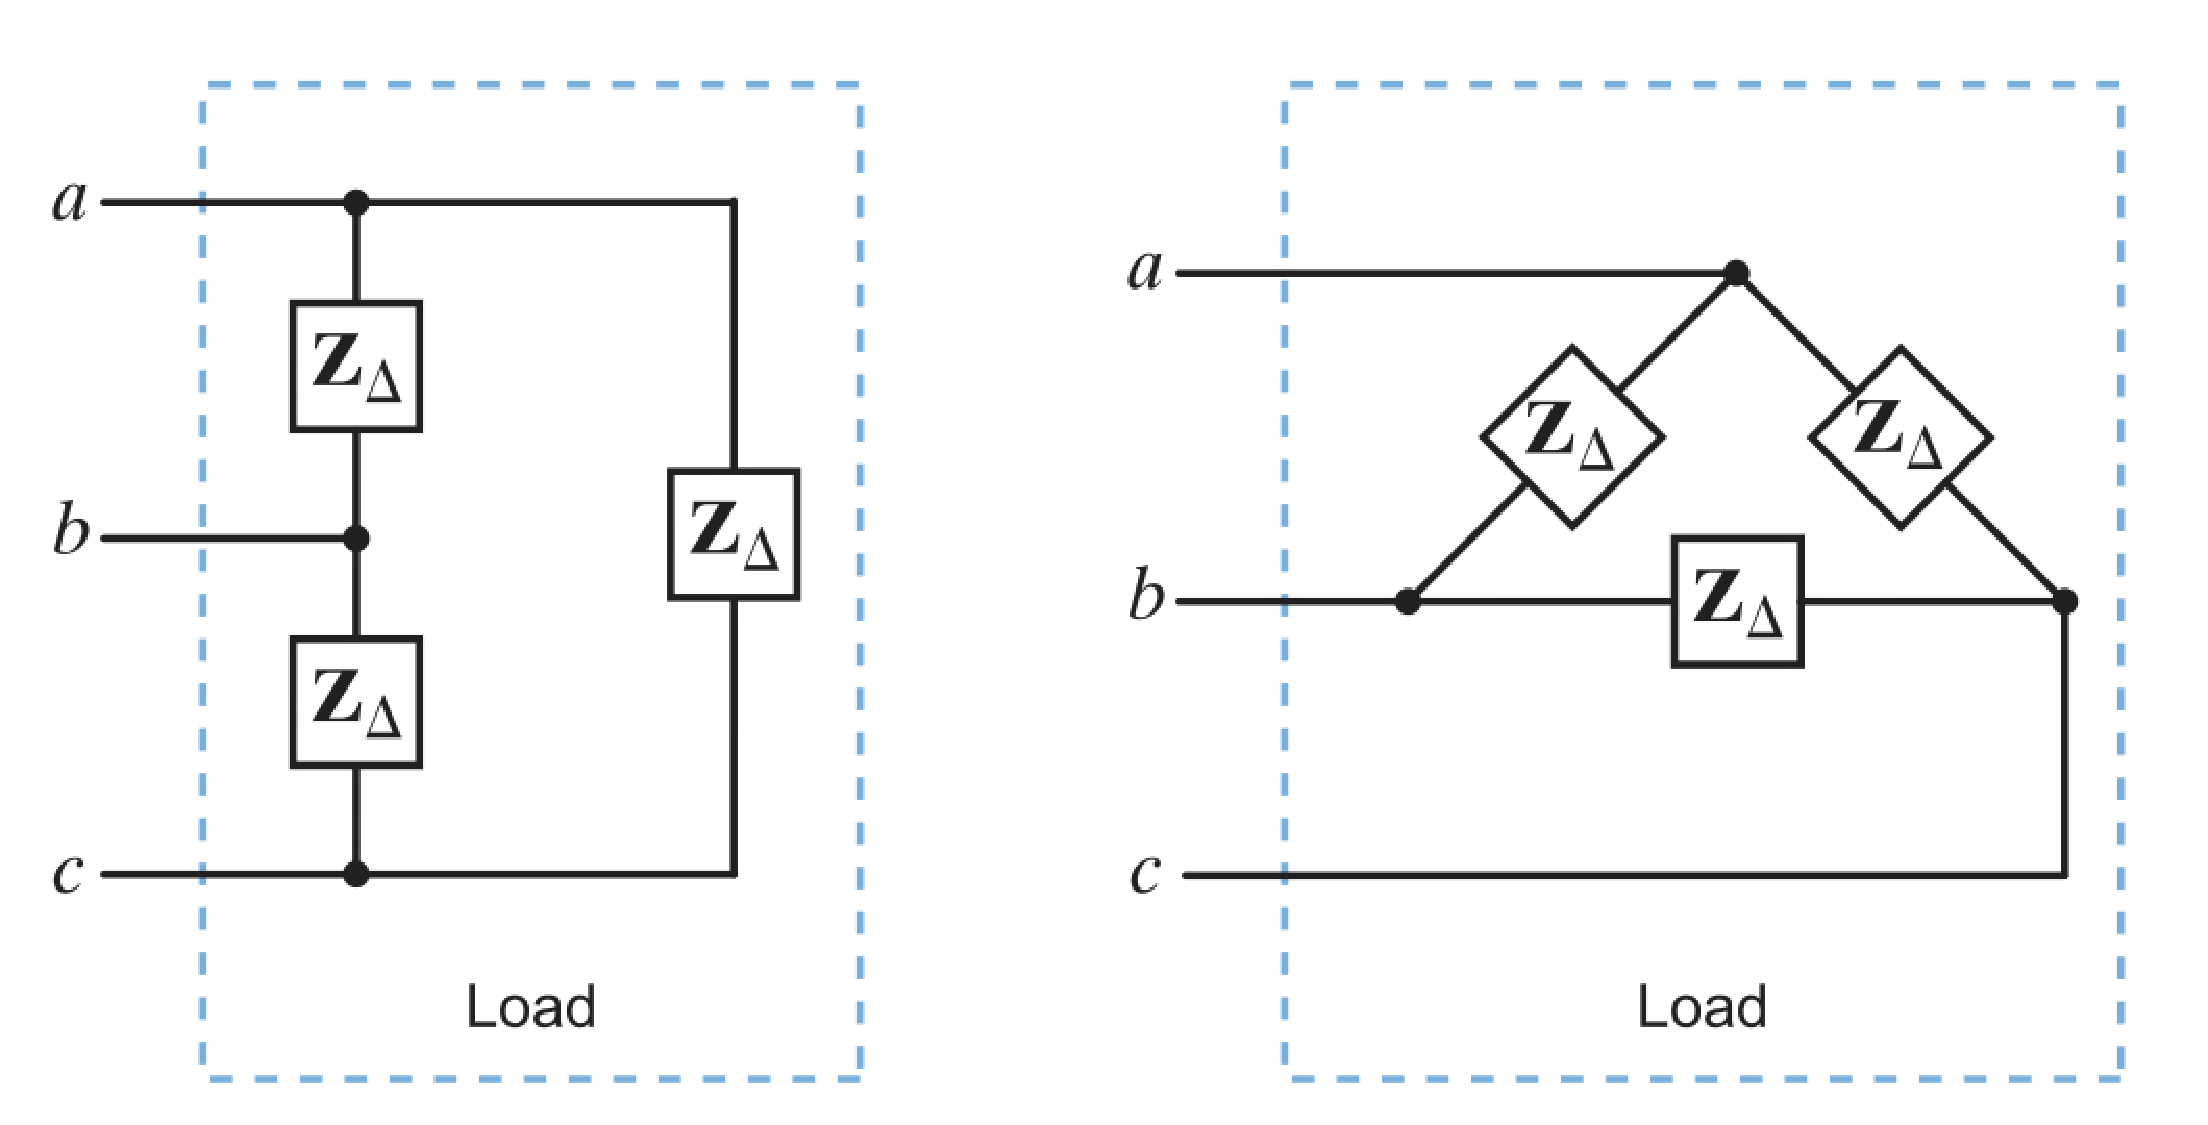
\includegraphics[height=2in]{delta_connection}
	\caption{Delta connected load}
	\label{fig:delta_connected_load}
\end{figure}

In a Y connected system, the line current for the phase \emph{a} is:
\begin{equation} \label{eq:balanced_tpIa}
	I_{a} = \frac{V_{an}}{Z_{y}} = \frac{V_{p}\angle_{\phi}}{Z_{y}}
\end{equation}
where $I_{b}$ and $I_{c}$ have the same magnitude but lag $I_{a}$ by 120\degree and 240\degree (respectively), since it is a balanced circuit. We can also denote that the neutral current is 0, since:
\begin{equation} \label{eq:balanced_tpIn}
	I_{n} = (I_{a} + I_{b} + I_{c}) = 0
\end{equation}

In a $\Delta$ connected system, since the line is connected between two phases, the line voltage that connects phase \emph{a} to phase \emph{b} ($V_{ab}$) depends on the phase voltage ($V_{p}$), being the $V_{ab}$ described by the equation \ref{eq:balanced_tpVab}, on page \pageref{eq:balanced_tpVab}.

The line voltages for $V_{bc}$ and $V_{ca}$ can also be defined the same way, being it described by equation \ref{eq:balanced_tpVbc} and \ref{eq:balanced_tpVca} (page \pageref{eq:balanced_tpVab}), respectively. 

The phase current for $I_{ab}$ is:
\begin{equation} \label{eq:balanced_tpIab}
	I_{ab} = \frac{V_{ab}}{Z_{\Delta}}
\end{equation}

The $\Delta$ impedance ($Z_{\Delta}$) is three times greater than the Y impedance ($Z_{Y}$).


% section sec:three_phase_systems (end)


\section{Three Phase Induction Motors} % (fold)
\label{sec:three_phase_induction_motors}

A motor is a machine that transforms electric energy in mechanical energy.
Such a machine can be implemented with the support of a DC power supply (DC Motor) or with a AC power supply (AC Motor).
In the AC Motor class, there are still two kind of motors - the synchronous motors and the asynchronous motors, being the latter also known as \acrfull{tpim}.


Thus, an \acrshort{tpim} can be implemented for a specific kind of phase voltage - single-phase, two-phase or three-phase.
By two-phases or three-phases (polyphase) it mean that the stator contains multiple distinct windings per motor pole, driven by corresponding time shifted sine waves.
Our focus will be on the \acrfull{tpim}.

These motors are  globally the most used, since they have several advantages over the single phase motors. For example, a three-phase motor is self starting due to the rotating magnetic field, while a single phase motor requires a capacitator and an auxiliary winding ~\cite{Ferreira1}.

\begin{figure}[htbp]
	\centering
	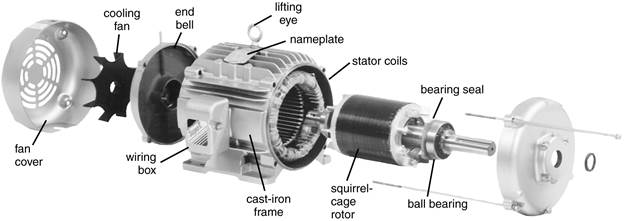
\includegraphics[height=2in]{ims}
	\caption{\Acrlong{ims}}
	\label{fig:ims}
\end{figure}

This kind of motors has been used, traditionally, in constant and variable-speed drive applications that do not offer fast dynamic processes. Because of the recent development of several new control techniques, this situation is changing. This is due to the fact that the \acrfull{ims} is much cheaper and more rugged than its competitors.

\subsection{Main Components}

The \acrshort{ims} is also known as asynchronous motor. This term \emph{asynchronous} is used because the rotational speed of the generated magnetic field is not equal to the rotational speed of the rotor. The term \emph{induction} is used because the rotor movements is due to the electromotive forces exercised by the generated magnetic field.
In figure \ref{fig:ims} (page \pageref{fig:ims}) you can see the several components of the \acrshort{ims}. You can see that the motor is composed by a fan, an end bell, a wiring box, a stator (and stator coils), a rotor (a squirrel-cage one) and bearings. The fan will mantain the motor at an appropriated temperature, while the stator will receive current from the power source connected to the motor and the rotor will rotate, supported by the bearings - creating mechanical movement.
In this section, we will only cover the stator and the rotor, which are the main components of the motors. 

\subsubsection{Stator}

The stator is the static part of the motor, which contains windings connected to a three-phase energy source. The stator represented in the figure \ref{fig:stator1} has six coils, and will generate a magnetic field with 2 poles when connected to a three-phase power source - since it has 6 coils (3 pairs), each pair of coils will connected to each phase of the three-phase power source supply.

These pairs of coils are connected in series for each phase of the power source supply, and corresponde to the opposite poles of an electromagnet. The figure \ref{fig:stator2} is an example of that magnet configuration, where each A, B and C is connected to its own phase of the three phase power supply.


\begin{figure}[htbp]
	\centering
	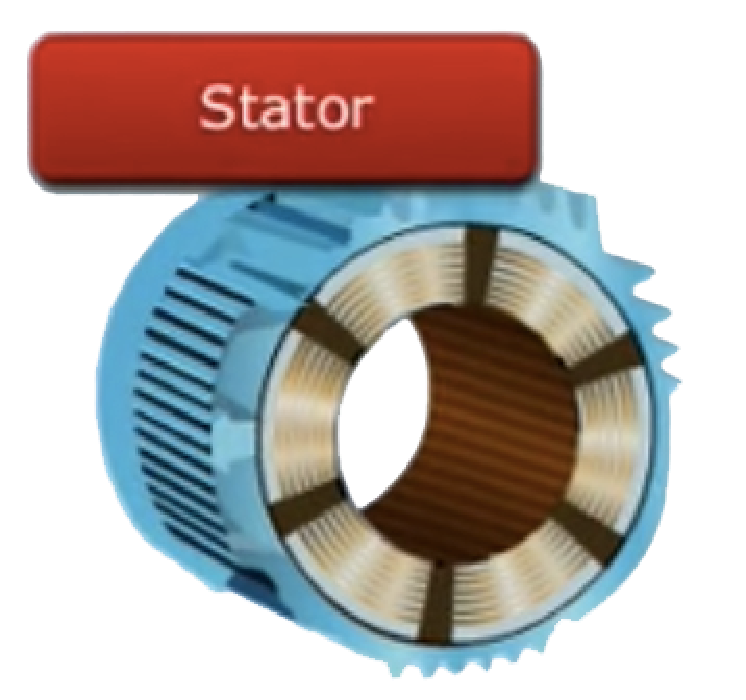
\includegraphics[height=2in]{stator_example}
	\caption{A stator}
	\label{fig:stator1}
\end{figure}

\begin{figure}[htbp]
	\centering
	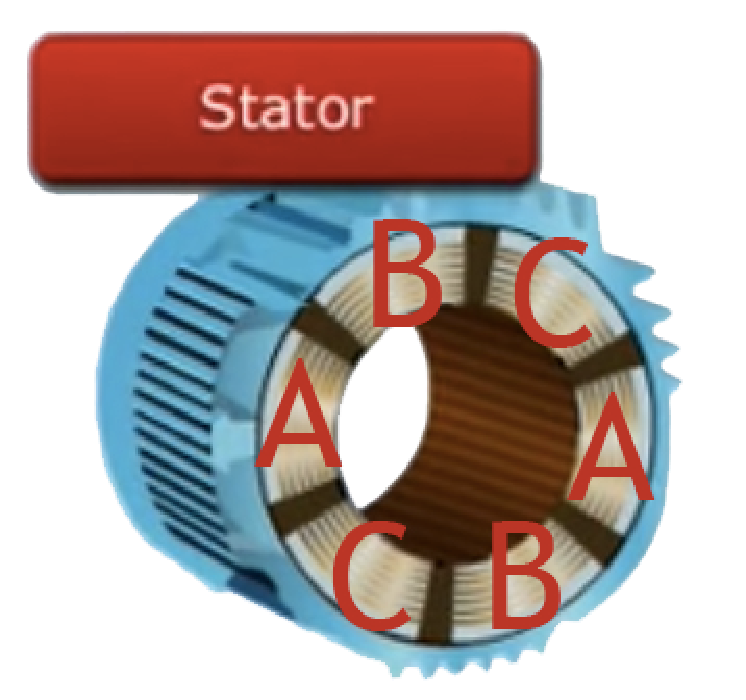
\includegraphics[height=2in]{stator_example2}
	\caption{A stator configuration model}
	\label{fig:stator2}
\end{figure}

In spite of the stators in the figures \ref{fig:stator1} and \ref{fig:stator2} have only 6 coils and generate a magnetic field with 2 poles, a stator can generate a magnetic field with 2, 4, 6, 8, 10, 12 or more poles - but motors with more than 12 poles are not normally used. For the stator to generate as many poles as needed, it must have a specific amount of coils configured in such a way so that the stator can generate the needed poles.


\subsubsection{Rotor}

The rotor is the rotative part of the motor and is inside the stator. In its essence, a rotor is a part of the motor where the magnetic field is induced so that it is pulled against the rotational magnetic field of the stator. Due to that purpose, the rotor has to be a conductor and has to have the hability to rotate.
The \acrshort{ims} has a squirrel cage rotor, but there is another type of rotor - the wound rotor. 

\begin{figure}[htbp]
	\centering
	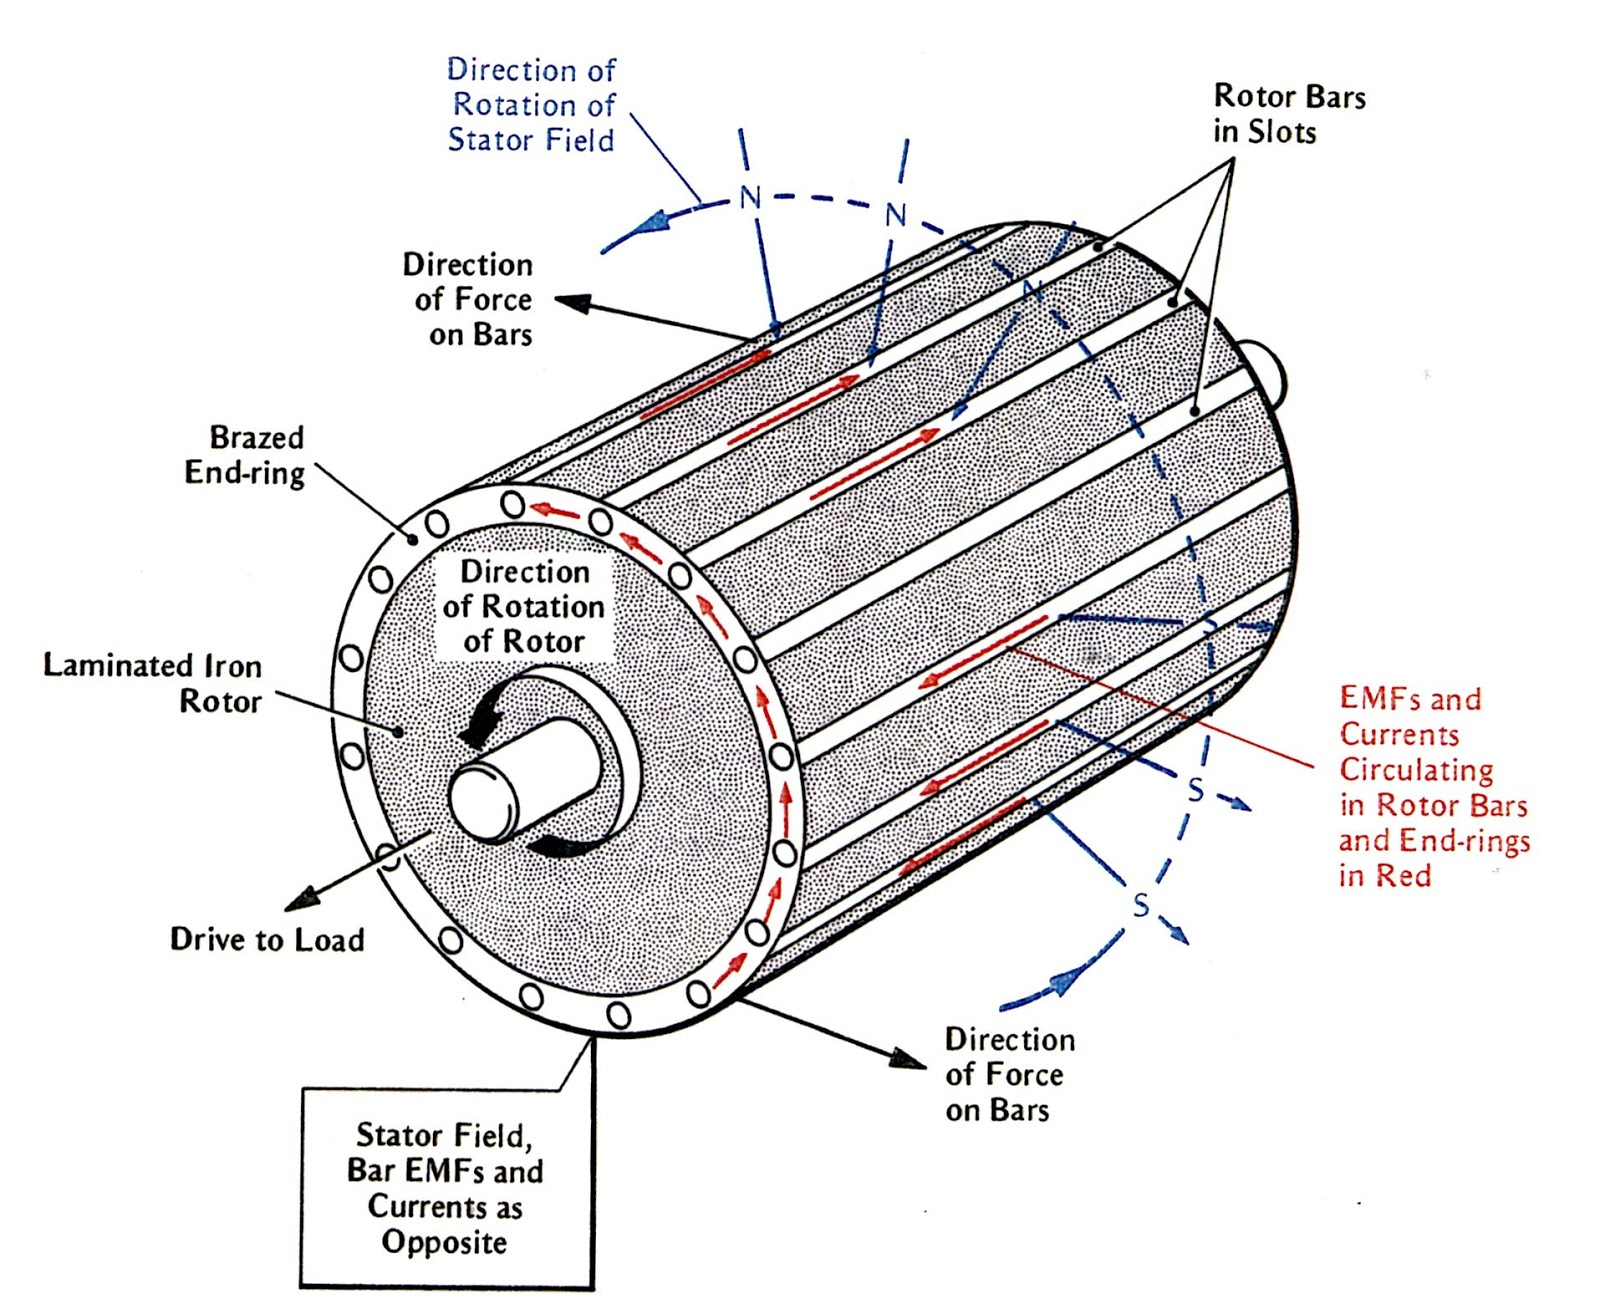
\includegraphics[height=3.5in]{squirrel_cage_rotor}
	\caption{A squirrel cage rotor}
	\label{fig:squirrel_cage_rotor}
\end{figure}

Most of the \acrshort{tpim} (up to 90\%) are of squirrel cage type.
As seen in figure \ref{fig:squirrel_cage_rotor}, this type of rotor consist of a cylindrical laminated core, having parallel slots on it. These parallel slots carry rotor conductors (represented as red arrows in figure \ref{fig:squirrel_cage_rotor}). In this type of rotor, heavy bars of copper, aluminum or alloys are used as rotor conductors instead of wires - as it would be in a wound rotor. 
The rotor slots are slightly skewed to achieve the following advantages:
\begin{enumerate}
  \item reduce locking tendency of the rotor, i.e. the tendency of rotor teeth to remain under stator teeth due to magnetic attraction
  \item increase the effective transformation ratio between stator and rotor
  \item increase rotor resistance due to increased length of the rotor conductor 
\end{enumerate}


\subsection{Working Principle}

The \acrfull{ims} - as well as the others \acrfull{tpim} - working principle is based on the generation of a rotating magnetic field by the stator. The windings that exist in the stator will create several electromagnetic coils, as shown in figure \ref{fig:stator2}. These coils are power supplied by a three phase AC source, which have the property of being sinusoidal - changing the value between positive and negative over time. This will generate a rotating magnetic field that will induce an electromotive force on the rotor, as seen in figure \ref{fig:rotating_3pmf}. 
This phenomena can also be view as an rotating magnet around the rotor. 


\begin{figure}[htbp]
	\centering
	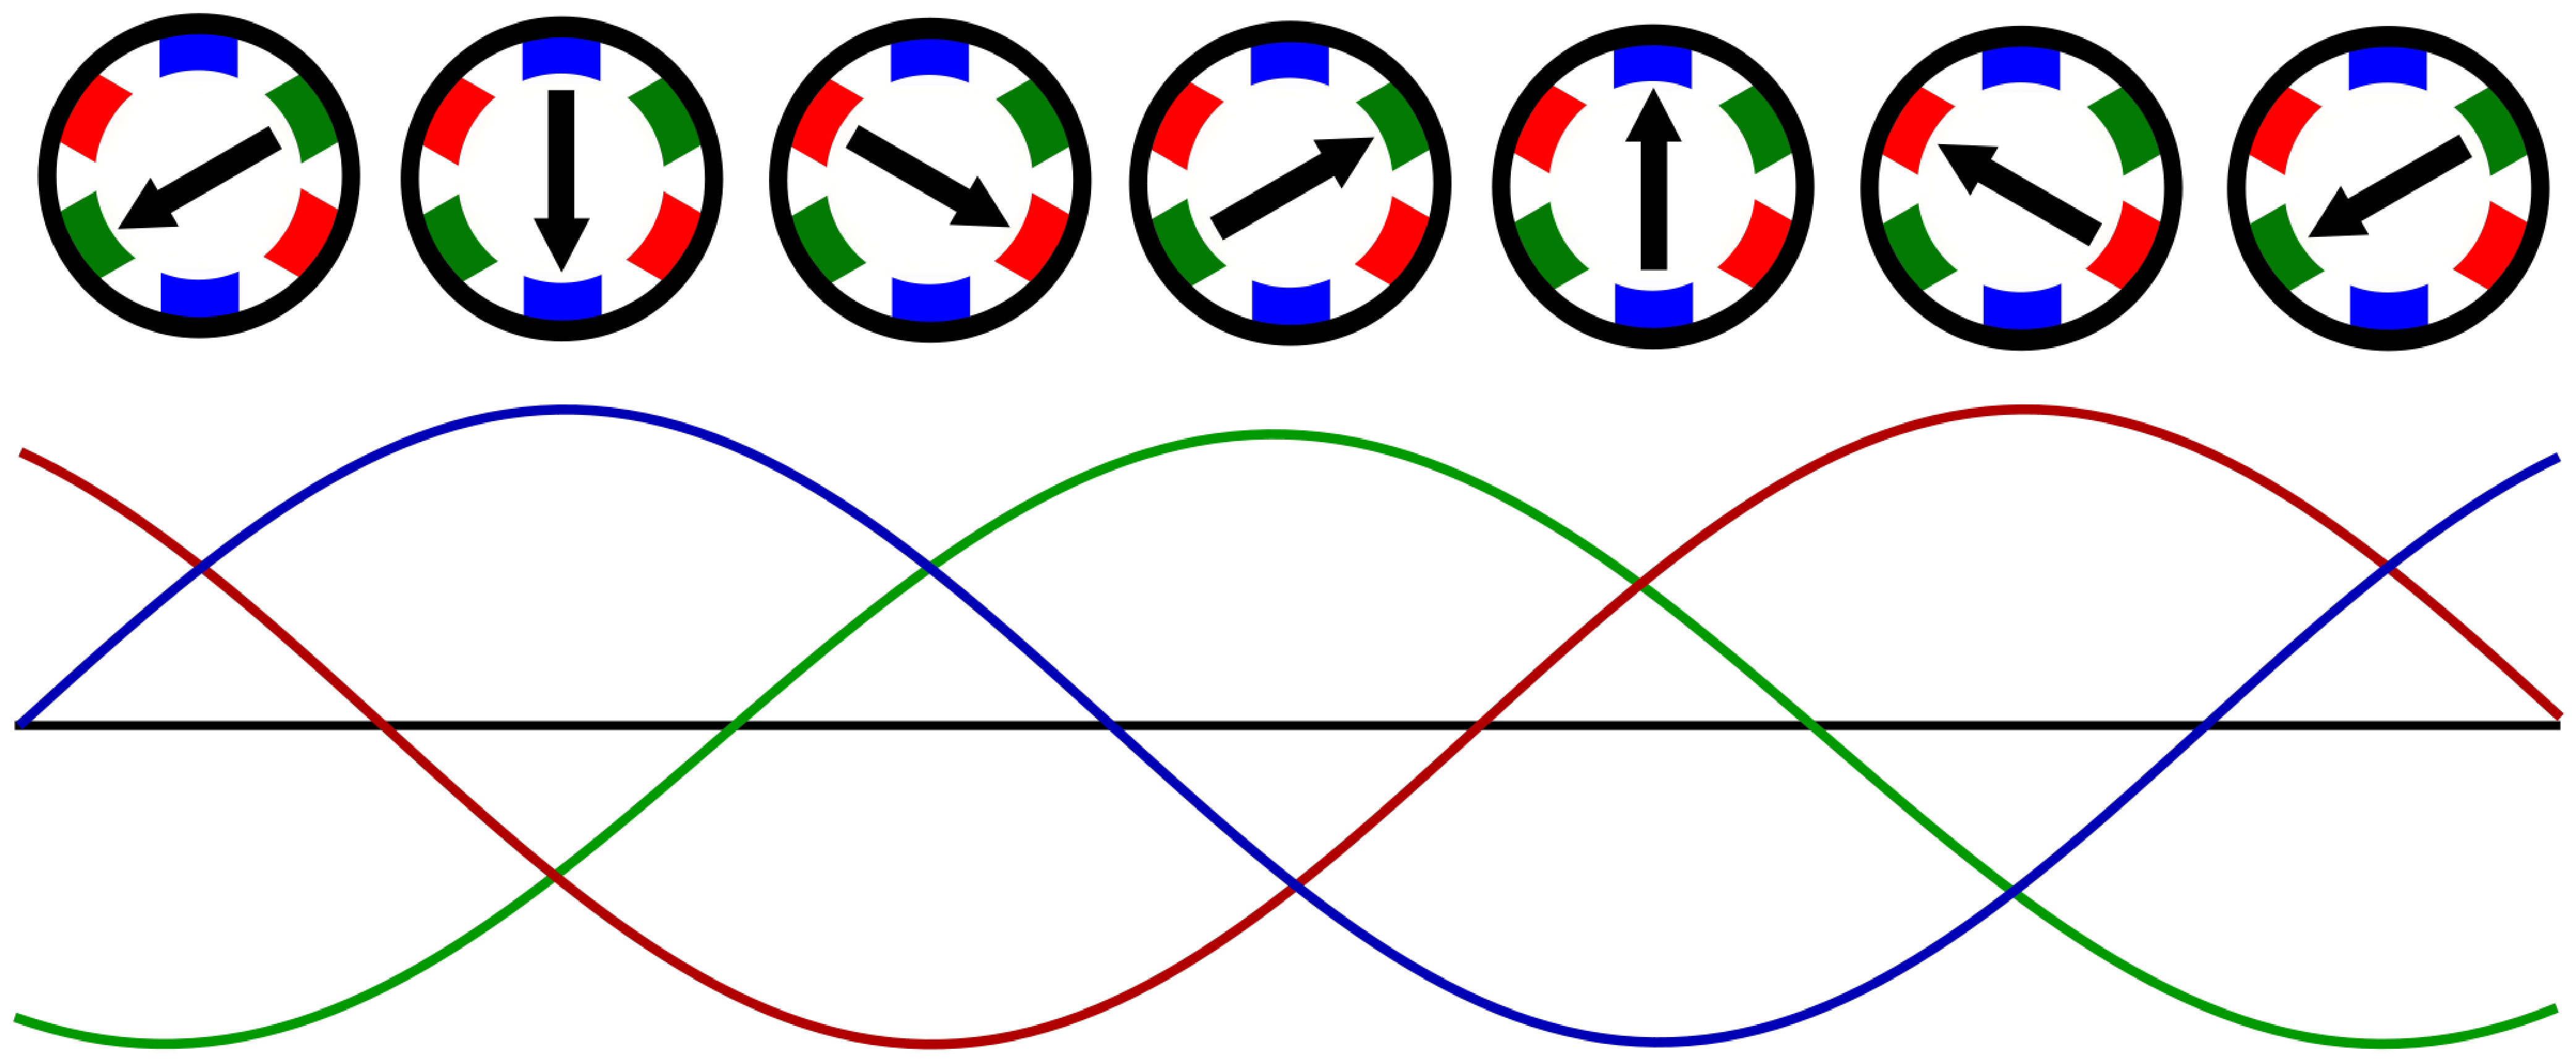
\includegraphics[height=2in]{Rotating-3-phase-magnetic-field}
	\caption{A rotating magnetic field with 6 coils and 2 poles}
	\label{fig:rotating_3pmf}
\end{figure}

\begin{figure}[htbp]
	\centering
	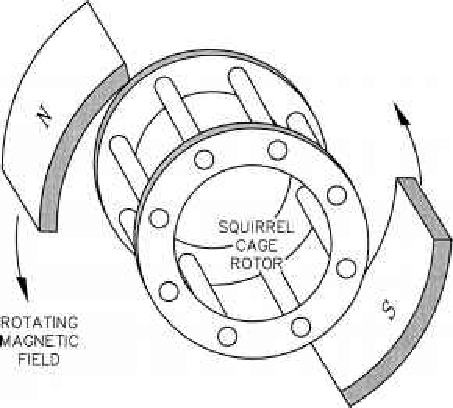
\includegraphics[height=2in]{rotating_squirrel_cage_rotor}
	\caption{Representation of the rotating magnetic field around the squirrel cage rotor}
	\label{fig:rotating_3pscr}
\end{figure}

Since the rotor has conductive components and the rotating magnetic field will create magnetic flux changes in the rotor, these magnetic flux changes will create a current in the rotor in such a way that it will create a magnetic field in the opposite direction of the magnetic flux change (Faraday-Lenz law).
This will create a magnet in the rotor that will try to align itself with the rotating magnetic field, as illustrated in figure \ref{fig:rotating_3pscr}.

Since the velocity in which the rotor rotates is lower than the rotational velocity of the magnetic field, the rotor will never align with the rotating magnetic field, creating the mechanical movement.

\subsection{Properties}

\subsubsection{Synchronous Speed}

The synchronous speed is the speed at which the rotational magnetic field rotates. This speed is constant, and its given by:

\begin{equation} \label{eq:synchronous_speed}
	 n_{s} = \frac{120f}{p}(rpm)
\end{equation}

\noindent where $f$ is the voltage frequency and $p$ is the number of poles in the stator.

From the expression \ref{eq:synchronous_speed} we can see that the greater is the pole quantity (always in pairs), the lower is the rotating magnetic field frequency.
Therefore, the max speed of an \acrshort{tpim} supplied by a 50hz power source is 3000rpm, due to the fact that the minimum value of poles number is 2.


\subsubsection{Slip}
In an \acrshort{tpim}, the rotor's rotational speed is not equal to the synchronous speed, since rotation at synchronous speed would result in no induced rotor current. This difference between synchronous speed and rotor speed is commonly referred to as the \emph{slip} of the rotor. We can measure this slip in rpm by subtracting the rotor speed to the synchronous speed, being it has follow:

\begin{equation} \label{eq:slip}
	 n_{s} - n
\end{equation}

\noindent where $n_{s}$ is the synchronous speed and $n$ is the rotor speed.

However, \emph{slip} is more usually expressed as a fraction of synchronous speed. The \emph{factional slip} $s$ is

\begin{equation} \label{eq:perc_slip}
	s = \frac{n_{s} - n}{n_{s}} 
\end{equation}

\noindent where $n_{s}$ is the synchronous speed and $n$ is the rotor speed.

The slip will depend of mechanical friction and the load. It is important to remember that the inductive reactance will depend on the speed difference between the inductor (stator) and the induced (rotor), and the bigger the difference then the bigger will be the inductive reactance. Therefore, the bigger the slip, the bigger will be the consumed current.

\subsubsection{Efficiency and Losses}

It is important to refer that slip is related to efficiency - the bigger the slip, the bigger the losses will be, thus lowering the motor's efficiency. The full-load slip gives an idea of the motor efficiency($\eta$), where:
\begin{equation} \label{eq:efficiency_max}
	\eta \leqslant 100\% - s
\end{equation}

The efficiency of a motor is greater the greater its power, being that the slip decreases with increasing power. Typical efficiency values for \acrshort{ims} are 80\% for 0.75kW power, 95\% for 100kW power and more than 98\% for high power motors.

\subsubsection{Torque}

The full-load torque of the motor can be known if the power and full-load speed are known, by the following expression:
\begin{equation} \label{eq:torque}
	T = \frac{P}{n}\times 9550
\end{equation}
where $T$ is measured in Newton.Meter (N.m), $P$ is power and is measured in KiloWatt (KW) and $n$ is the rotor speed and is measured in rpm.

When the motor operates at full-load, the generated torque is the necessary to maintain the rotation of the load at full-load speed. However, at start, the necessary torque has to be bigger than the force imposed by the load, as seen in figure \ref{fig:torque_speed_curve}, where the rated torque is the maximum torque that the motor can safely apply continuously to the load at any speed within the rated speed range of the motor.

\begin{figure}[htbp]
	\centering
	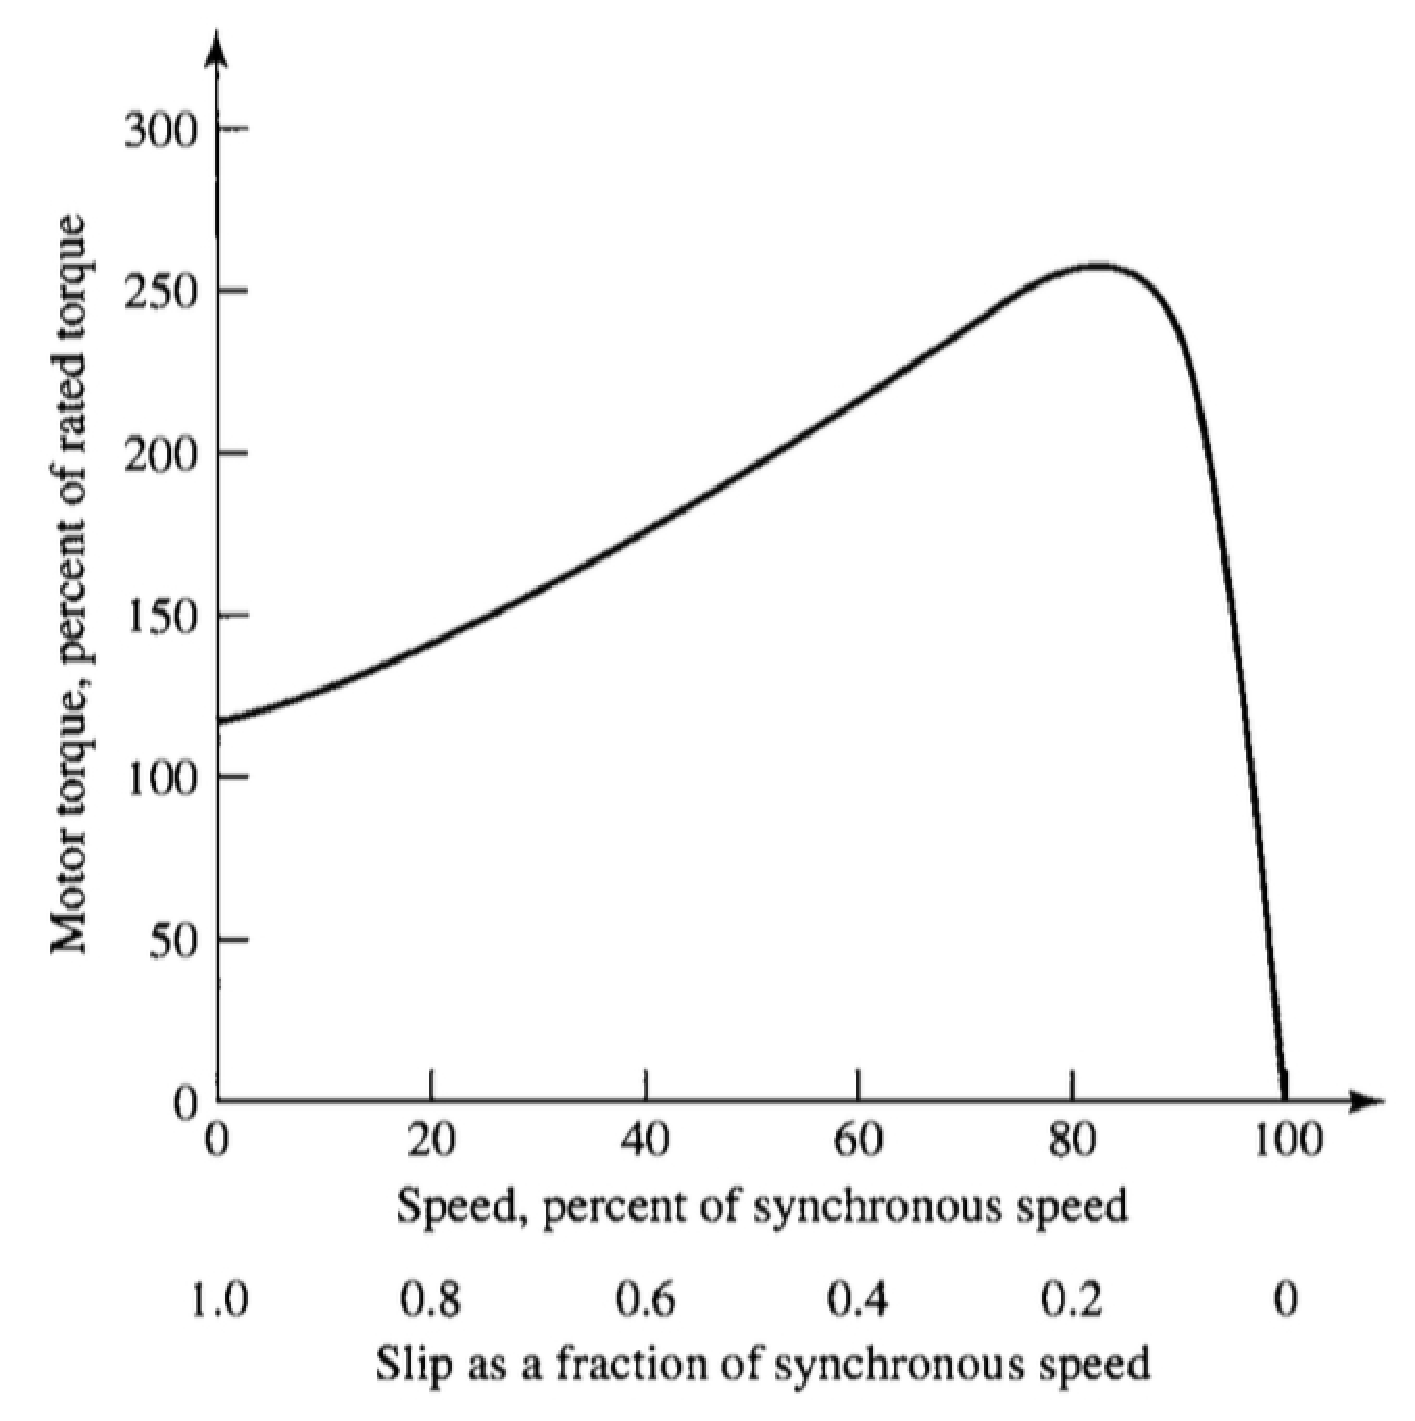
\includegraphics[height=4in]{torque_rotor_speed}
	\caption{Typical \acrshort{tpim} torque-speed curve for constant voltage, constant frequency operation}
	\label{fig:torque_speed_curve}
\end{figure}

\subsubsection{Motor Start}

At the start, the rotor is stationary ($n = 0$) and the slip (equation \ref{eq:perc_slip}) is 1. Then, the field produced by the rotor currents revolves at the same speed as the stator field, creating a starting torque. 
This torque will tend to turn the rotor in the direction of rotation of the stator-inducing field. If this torque is sufficient to overcome the opposition to rotation created by the shaft load, the rotor will come up to its operating speed - as seen in figure \ref{fig:torque_speed_curve}.

If an induction motor is directly switched on from the supply it takes 5 to 7 times its full load current and develops a torque which is only 1.5 to 2.5 times the full load torque. 
This large starting current can have adverse effects to the motor (deteriorating insulation due to overheating) as well as to the electrical installation (triggering the protection device), where a large voltage drop in the line can affect the operation of other devices connected to the same line.

Therefore, various starting methods of induction motors were developed, such as:

\begin{itemize}
  \item 
  \emph{Using Primary Resistors}, which are applied in series in the stator's windings. Due to Joule effect losses, this method is anti-economic.
  \item 
  \emph{Auto-Transformers} are used to help the motor start by changing the voltage. Due to the auto-transformer price, this is an expensive method.
  \item 
  \emph{Star-Delta Starter} is a device that initially connects the stator in Y configuration and after a certain velocity ($n$), it changes that connection to a $\Delta$ configuration, raising the voltage applied to the windings.
  \item 
  \emph{Power Converter} is a device that can control motor speed as well as the motor start through frequency variation.
\end{itemize}

\subsubsection{Motor Speed Control}
\acrshort{ims} speed control can be done using several methods

\begin{itemize}
  \item 
  The stator can be projected in such a way that alternating the coil's windings leads to a different number of poles. In spite of being a robust and efficient method, it has the downsides of the resulting velocities being only discrete (as it can be infer from the equation \ref{eq:synchronous_speed}) and the stators capable of this are more expensive and complex. 
  \item 
  It is also possible to use a variable frequency voltage device (power converter) as a voltage provider for the motor. As you can see in equation \ref{eq:synchronous_speed}, the value of the frequency will change the speed of the motor.
  \item 
  A voltage converter can also be used, ranging the magnitude of the voltage. Once the torque is proportional to the voltage, changing the voltage magnitude will change the motor speed.
  \item 
  There is also the possibility to use the last two methods - ranging the voltage frequency and ranging the voltage magnitude.
\end{itemize}

\section{Relevance and Landscape of Three Phase Induction Motors} % (fold)
\label{sec:tpin_relevance}

\acrshort{em}s are an important component of \acrshort{emfs}, which are part of the industrial equipments' great majority. Due to its characteristics, \acrshort{em}s can be found in applications as diverse as industrial fans, blowers, pumps, compressors, conveyors, lifts, households appliances, power tools, etc. 
Such applications lead to an high consumption of electrical energy.

Worldwide, \acrshort{em} are responsible for the consumption of 30-40\% of electrical energy, while in developed countries this values raises to 50-60\% and in European Union to 70-75\%, making them one of the most important electrical charges, being responsible for 13\% of $CO_{2eq}$. 
Due to its relatively low price, good efficiency and high availability, \acrshort{ims}  are the most used electric motors in the market of power from 0.75KW - representing 85-90\% of the installed motors in the industry. 

Still, there are several types of electric motors in the industry. Above the 0.75KW of power, the motors normally used are \acrfull{tp} \acrshort{ac} and commutated \acrshort{dc} with \acrshort{tp} electric controllers.
In the \acrshort{tp} \acrshort{ac} domain, in addition to \acrshort{ims}, we also have \acrfull{wrtpim}, \acrfull{wrtpim}, \acrfull{pmsm} and \acrfull{rm}. 

For powers above 0.75KW, conventional \acrshort{dc} motors are bound to disappear in the industry due to its low availability and efficiency. However, in the \acrshort{dc} domain, there are two types of motors widely used - \acrfull{bldc} and \acrfull{srm}, both requiring electric controllers.

Nowadays, \acrshort{ims}'s power can go to 5MW. However, most of these motors have a power ranging from 0.75KW to 375KW. 

\acrshort{wrtpim} are used for power needs above 1MW, but these are being gradually replaced for \acrshort{ims} supplied by \acrfull{esv}. Since \acrshort{wrtpim} have brushes, bearings and windings in the rotor, which leads to a lower availability and an higher cost comparing to the \acrshort{ims}. This gradual change is happening to only because of this lower availability and higher cost, but also because of the advances in the  \acrfull{esv} domain, which allow changing the torque-speed curve of \acrshort{ims}.

\acrshort{pmsm} are used in low-power applications (usually until 15KW), having an high efficiency curve and an excellent power factor, however needing an electric controller to operate. In spite of its power/height ratio is better than \acrshort{ims}'s, the \acrshort{pmsm} price plus the electric controller is higher than the \acrshort{ims} cost, being this the main disadvantage of \acrshort{pmsm} relatively to \acrshort{ims}- if the requirement is constant speed.

\acrshort{rm} are normally used in power needs ranging from 5KW a 700KW and are an interesting technology on the efficiency/power factor point of view, being its cost higher than the \acrshort{ims}. This a disadvantage if the requirement is constant speed.

\acrshort{pmsm} with squirrel-cage rotor are a promising technology that combine high efficiency and the characteristic \acrshort{pmsm} power factor, as well as line-start capability characteristic of \acrshort{ims} - removing the need of an electric controller.
However, due to several technical problems related to the motor start and sync, there aren't commercial models available for power above 3KW - restraining this way the power of the commercialized models from 0.3KW to 3KW.

Due to the previously identified points, it is concluded that the most relevant motor for the next years is the \acrshort{ims}, being this the target motor type of this thesis.

\section{Three Phase Induction Motors' Operation} % (fold)
\label{sec:Three_phase_induction_motors_maintenance_and_lyfe_cycle}

In most of the cases, the \acrshort{ims}'s \acrfull{lcc} can go up to 90\% of its exploration cost, which directly influences their performance and availability. Both of these measures can be optimized through appropriated maintenance strategies, ensuring appropriated operating conditions and including the power supply quality. Nevertheless, motor failures or malfunctions can still occur.

\subsection{Life-cycle cost}
\label{subsec:life_cycle_cost}

The \acrshort{lcc} of \acrshort{em} is the cost's sum of acquisition, exploration, maintenance and shutdown, as illustrated in figure \ref{fig:lcc}. If we want to be more precise, the outage cost of a motor can also be included in its \acrshort{lcc}, due to production losses and inactive labor for example.


From the components of the \acrshort{lcc}, the two biggest costs are the exploration cost and the maintenance cost - as shown in figure \ref{fig:costsOflcc}.

\begin{figure}[htbp]
	\centering
	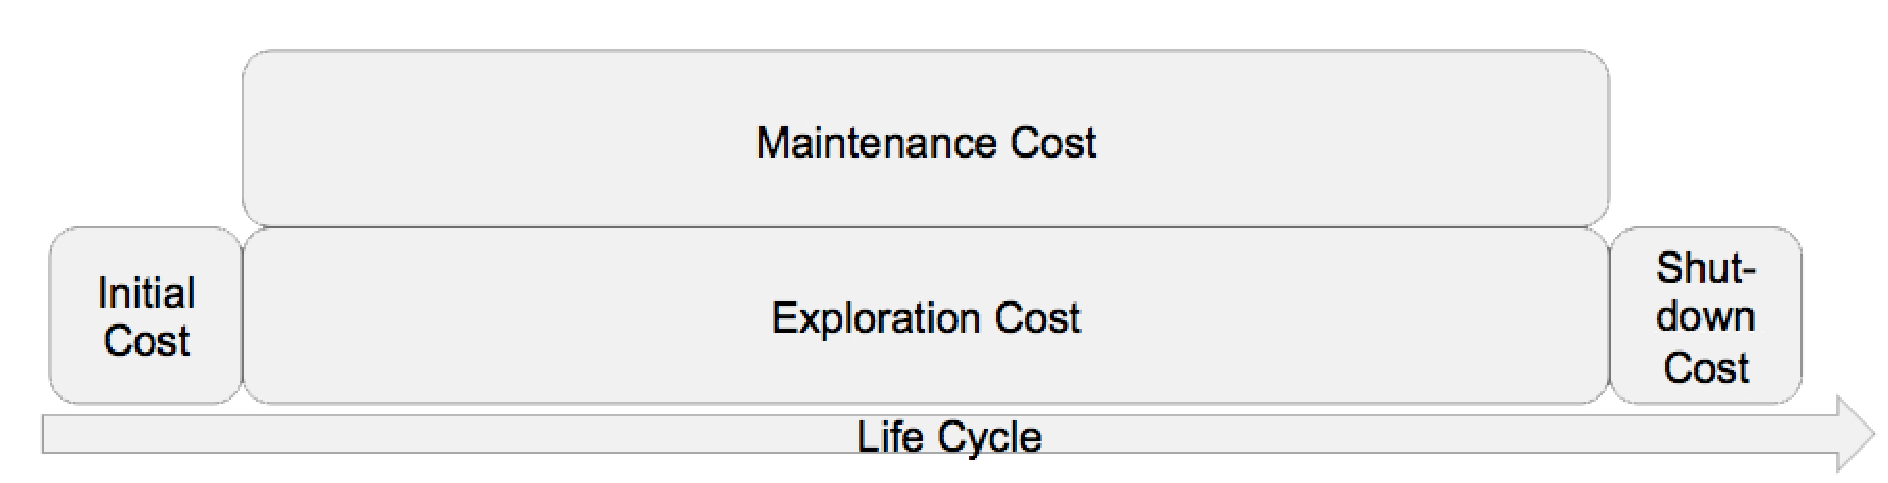
\includegraphics[height=1.5in]{lcc}
	\caption{Life Cycle cost components}
	\label{fig:lcc}
\end{figure}

Active power has a direct influence in the contracted/taken power and peak power, which have a specific cost associated in the electric bill. Therefore, bigger efficiency means less energetic costs.
The low motor's availability may have very significant indirect costs. When the motor fails unexpectedly, there are significant costs associated to its unplanned stop due to possible system stops, production losses, inactive labor, delivery failures and possibly lost of clients, transport of the motor to the repairer, motor repair, etc. 
Generally, the investment in \acrshort{ims}'s efficiency, power factor and availability improvements is largely compensated by the benefits that come from it.
 
\begin{figure}[htbp]
	\centering
	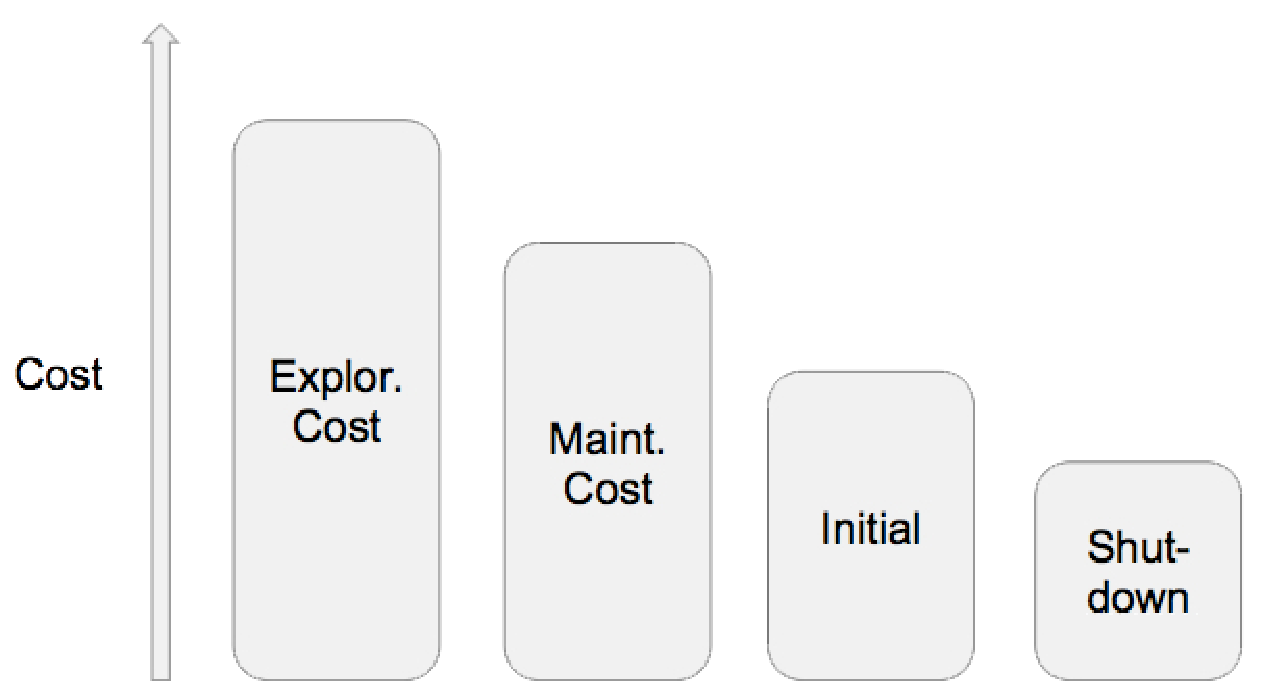
\includegraphics[height=2in]{costsOflcc}
	\caption{Life Cycle costs quantity}
	\label{fig:costsOflcc}
\end{figure}

\subsection{Maintenance Strategies}
\label{subsec:maintenance}

Maintenance strategies are developed in order to ensure maximum availability, efficiency, production processes' security, preserve equipments and improve the production quality. Generally, if the additional cost paid for maintenance is equal or less than the reduction in motors' exploration cost, then that investment is economically good.

The motors' manufacturers typically provide a set of recommendations concerning its maintenance and conservation, where these recommendations should be followed.

Nevertheless, a suited maintenance plan consists on a preventive maintenance component as well as on a predictive maintenance component.

\subsubsection{Corrective Maintenance}
\label{subsubsec:corrective_maintenance}

This maintenance strategy acts when the equipment has already broke down. It focus on restoring the equipment to its normal operating condition, but it is also possible to choose to replace the motor instead of restoring the broken one. 

If the repair is done, then it is also possible to apply some preventive maintenance protocols. This way, in order to avoid a new posterior motor stop, the components that are scheduled to be object of a preventive maintenance strategy are replaced.

Several independent studies have shown that the \acrshort{ims} repairs leads to the efficiency reduction in 1\% to 4\%. It may also lead to an availability reduction and to the change of torque-speed curve, which degrades the motor's performance.


\subsubsection{Risk based Maintenance}
\label{subsubsec:risk_based_maintenance}

This maintenance strategy is the base maintenance procedure applied to all the motors in which the protocol may take into account the motor's lubrication, windings replacement, motor's surface cleaning and check of the electric connectors.

The frequency in which this maintenance strategy is applied may vary, depending on the motor's importance in the industrial process, as well as its operation conditions - having special attention on the environment conditions like humidity, dust and temperatures.

\subsubsection{Preventive Maintenance}
\label{subsubsec:preventive_maintenance}

This maintenance strategy presumes the periodic replacement of some motor's components, independently of their actual state of degradation.
This is based on statistical analysis of components' life duration.

However, since the major part of the replaced components are still in a good state, there is always a waste factor associated with this maintenance strategy to take into account. Therefore, it is acceptable that this kind of maintenance may only be applied to critical motors of the system.	


\subsubsection{Predictive Maintenance}
\label{subsubsec:predictive_maintenance}
%This strategy can be viewed as a sub-area of preventive maintenance, in that some malfunctions signals may trigger some action in the motor.
The main goal of this maintenance strategy is to provide timely malfunction signals, so that the probability of an outage may be reduced. In doing so, not only we are providing information of the motor's status, we are also reducing some malfunctions' cost. 
If the malfunctions are detected in an early stage then the repair actions tend to be less costly, not only because it is possible to timely plan the repair, as well as the malfunction tend to stay contained to its original location, not spreading to other areas of the motor. 

This strategy presents some characteristics to accomplish its goals, as for the use of non invasive techniques (so that it is not required to stop the motor) and in the attempt to eliminate corrective maintenance. 


\subsection{Motor failures}
\label{subsec:motor_failures}

Over the years, several surveys (~\cite{Bonnett2010}, ~\cite{Thorsen1995}, ~\cite{Mccoy1986}, ~\cite{Bonnett1992}) have been made targeting the failure analysis of induction motors (small, medium and large), leading to similar values in the principal fault's categories and a better understanding about the failure's cause.

In spite of the variety of sources of machine faults (figure \ref{fig:Sources_im_failures}), these studies have converge in the main sources of failures and shown similar values about the frequency in which they happen, as shown in table \ref{tab:failure_distribution}. A drilled down distribution can be seen in the table \ref{tab:failure_distribution_drilldown} according to ~\cite{Mccoy1986}.

These same studies also show that the failure distribution varies within industries, application and power category - since ~\cite{Bonnett2010} and ~\cite{Thorsen1995} target machines in the petrochemic and oil industry, and ~\cite{Mccoy1986} targets machines in utility applications.


In these same studies it was also determined that a given population of motors had an average failure rate of 0.0708 failures per unit, per year (FPU) for general industry ~\cite{Reliability1987} and 0.035 FPU for maintenance-intensive industries such as utilities ~\cite{Mccoy1986}.

\begin{table}[]
\centering
\caption{Failure Category Distribution}
\label{tab:failure_distribution}
\begin{tabular}{ccccc}
\multicolumn{1}{c}{\textbf{}} & \multicolumn{1}{c}{\textbf{\% Bearings}} & \multicolumn{1}{c}{\textbf{\% Stator}} & \multicolumn{1}{c}{\textbf{\% Rotor}} & \multicolumn{1}{c}{\textbf{\% Others}}  \\
~\cite{Bonnett2010}  & 51 & 16 & 7 & 26 \\ 
~\cite{Thorsen1995}  & 51 & 16 & 7 & 26 \\
~\cite{Mccoy1986} 	 & 41 & 36 & 9 & 14 \\
~\cite{Bonnett1992}  & 41 & 37 & 10 & 12 \\                              
\end{tabular}
\end{table}


%\todo[inline]{Ter a figura ou ter as tabelas?}

\begin{figure}[htbp]
	\centering
	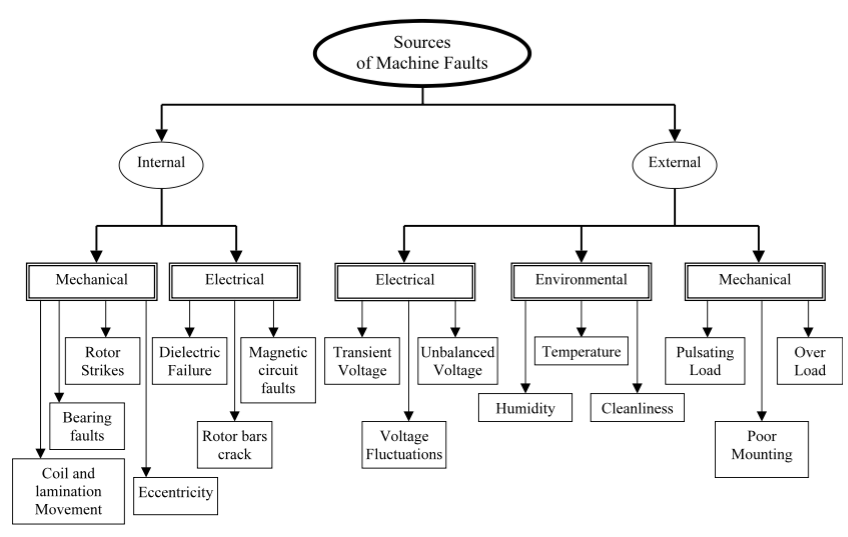
\includegraphics[width=\textwidth ]{Sources_im_failures}
	\caption{Sources of induction motor failures}
	\label{fig:Sources_im_failures}
\end{figure}

\begin{table}[htbp]
\caption{Failure Category Distribution Drilldown}
\label{tab:failure_distribution_drilldown}
\begin{tabular}{cc}
\multicolumn{1}{c}{\textbf{Bearings Related}} & \multicolumn{1}{c}{\textbf{41\%}} \\
Sleeve Bearings & 14\% \\
Anti-Friction Bearings  & 9\% \\
Oil Leaks & 6\% \\
Thrust Bearing & 5\% \\
Bearing seals & 3\% \\
Oil System & 1\% \\
Other & 3\%
\end{tabular}
\begin{tabular}{cc}
\multicolumn{1}{c}{\textbf{Stator Related}} & \multicolumn{1}{c}{\textbf{36\%}} \\
Grounding Insulation & 22\% \\
Turn Insulation  & 4\% \\
Bracing & 3\% \\
Wedges & 1\% \\
Frame & 1\% \\
Cable & 1\% \\
Connections & 1\% \\
Other & 3\%
\end{tabular}
\begin{tabular}{cc}
\multicolumn{1}{c}{\textbf{Rotor Related}} & \multicolumn{1}{c}{\textbf{9\%}} \\
Cage & 4\% \\
Shaft  & 2\% \\
Core & 1\% \\
Balance Weight & 1\% \\
Other & 1\%
\end{tabular}
\end{table}


\section{Turn Insulation Faults}
\label{sec:turn_insulation_faults}

Short-circuit faults form 26\% of the faults occurring in \acrshort{ims}, as stated in Table \ref{tab:failure_distribution_drilldown}. By short-circuits, we are counting the turn insulation and ground insulation faults categories.
It has been reported that most short-circuit faults begin as interturn faults ~\cite{Bonnett1992}, which occur due to insulation failures but develop into more serious faults very quickly.
Insulation failures are attributed to different reasons, with the primary reason being excessive thermal stresses.Other reasons for insulation failure include voltage stresses, aging, vibrations, or mechanical handling during assembly.

Interturn faults are faults that happen in between turns of a winding, as shown in figure \ref{fig:insulation_faults}.

\begin{figure}[htbp]
	\centering
	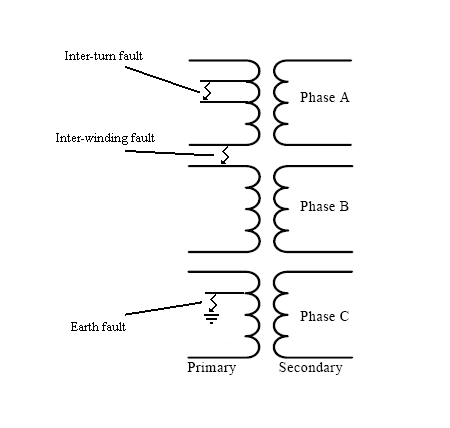
\includegraphics[width=0.5\textwidth ]{insulation_Faults}
	\caption{Types of insulation faults. Source: http://www.openelectrical.org/wiki/images/b/b9/Transformer\_Faults.png}
	\label{fig:insulation_faults}
\end{figure}

Since the current now have a shorter circuit, the consequence of this fault is that the \acrfull{mmf} will decrease, since now it has less turns. Further, the current in the shorted turns produces also an \acrshort{mmf} which opposes against the main \acrshort{mmf} generated by the phase windings.


If not timely detected, the fault progressively spreads and the fault current increases, increasing as well the thermal stress in its surroundings. The small inter-turn short-circuit can degenerate into a catastrophic interwinding (or phase-to-phase) short-circuit, or even in an earth (or phase-to-ground) short-circuit (also shown in figure \ref{fig:insulation_faults}). The earth fault is referred in the table \ref{tab:failure_distribution_drilldown} as grounding insulation.

This processes develops rather quickly and appropriated measures must be taken to contain the fault.